











\chapter{Profiling Python bytecode} % for fun and profit
\label{chap:profiling-bytecode}






\chapter{Specialising and optimising xDSL pattern rewriting}
\label{chap:specialising-optimising-pattern-rewriting}

\section{Micro-benchmarks}

% Hook
% Argument
% Link

\subsection{Operation trait checks}

% Hook
Chapter \ref{chap:measuring-compiler-performance} measured a slow-down of approximately $130\times$ from MLIR to xDSL for trait checking micro-benchmarks (\autoref{tab:ubenchmark-trait-checks}).
% Argument
There are two factors which contribute to this slow-down. The first is the inherent overhead incurred by the interpreter loop and data structures in Python's dynamic language runtime. The second is differences in implementation between xDSL and MLIR.
% Link
Examining this micro-benchmark in detail allows us to decouple the performance contributions of the implementation and language runtime.
% , and provides insight into the impact of dynamism on user-extensible compiler framework workloads.

\begin{figure}[H]
    \begin{subfigure}[b]{0.45\textwidth}
       \centering
        \begin{minted}[fontsize=\footnotesize]{python}
            @classmethod
            def has_trait(
                cls,
                trait: type[OpTrait] | OpTrait,
                *,
                value_if_unregistered: bool = True,
            ) -> bool:
                from xdsl.dialects.builtin import UnregisteredOp
        
                if issubclass(cls, UnregisteredOp):
                    return value_if_unregistered
        
                return cls.get_trait(trait) is not None
        \end{minted}
        \footnotesize\vspace{1.5em}
        \caption{Outer \mintinline{python}{has_trait} method.}
        \label{listing:ubenchmark-trait-checks-xdsl-has}
    \end{subfigure}
    \hfill
    \begin{subfigure}[b]{0.45\textwidth}
        \centering
        \begin{minted}[breakanywhere,fontsize=\footnotesize]{python}
            @classmethod
            def get_trait(
                cls,
                trait: type[OpTraitInvT] | OpTraitInvT
            ) -> OpTraitInvT | None:
                if isinstance(trait, type):
                    for t in cls.traits:
                        if isinstance(t, cast(
                            type[OpTraitInvT], trait
                        )):
                            return t
                else:
                    for t in cls.traits:
                        if t == trait:
                            return cast(OpTraitInvT, t)
                return None
        \end{minted}
        \caption{Inner \mintinline{python}{get_trait} method.}
        \label{listing:ubenchmark-trait-checks-xdsl-get}
    \end{subfigure}
    \vspace{1em}
    \captionsetup{name=Listing}
    \caption{xDSL methods implementing trait check functionality.}
    \label{listing:ubenchmark-trait-checks-xdsl}
\end{figure}

% Hook
In order to distinguish between the slow-down incurred by the language runtime as opposed to each approach's implementation, we leverage tracing profilers to examine the call stacks of the micro-benchmarks.
% Argument
In the xDSL implementation of \mintinline{python}{has_trait} (Listing \ref{listing:ubenchmark-trait-checks-xdsl}), we can see that approximately half of the operation is spent checking if the operation subclasses \mintinline{python}{UnregisteredOp} (\autoref{fig:ubenchmark-hastrait-xdsl-viztracer}).
Furthermore, \mintinline{python}{has_trait}s sub-invocation \mintinline{python}{get_trait} further incurs overhead with \mintinline{python}{isinstance} checks, \mintinline{python}{cast}ing and constructing iterators (\autoref{fig:ubenchmark-gettrait-xdsl-viztracer}).
% Link
This demonstrates that a significant proportion of the slow-down in xDSL's \mintinline{python}{has_trait} method is as a result of implementation details, as opposed to inherent limitations of Python's runtime.

\begin{figure}[H]
    \centering
    \begin{subfigure}[b]{\textwidth}
        \centering
        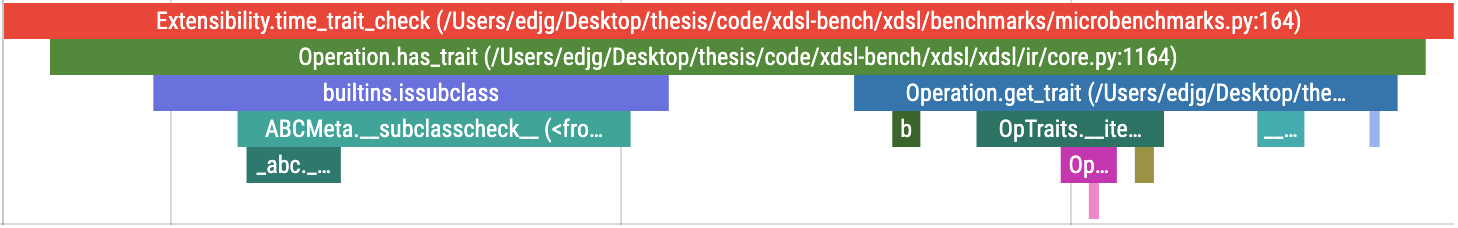
\includegraphics[width=\textwidth]{images/14_understanding_compiler_performance/trait_checks/hastrait_xdsl_viztracer.png}
        \caption{Checking for \mintinline{python}{UnregisteredOp}s constitutes around half of \mintinline{python}{has_trait}s runtime.}
        \label{fig:ubenchmark-hastrait-xdsl-viztracer}
    \end{subfigure}
    \begin{subfigure}[b]{\textwidth}
        \centering
        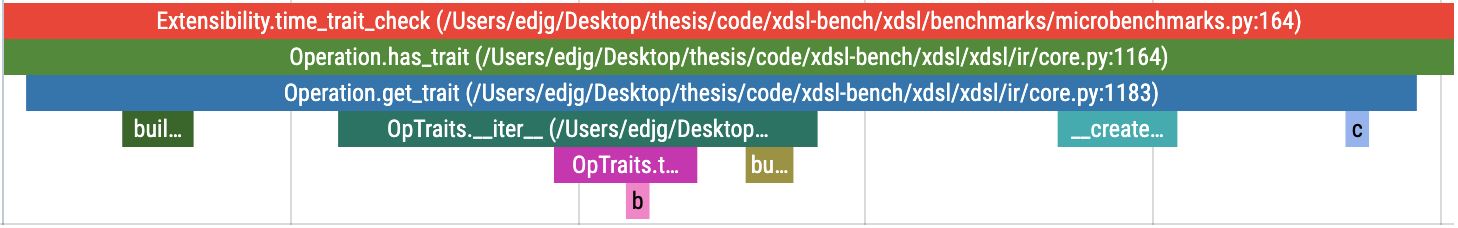
\includegraphics[width=\textwidth]{images/14_understanding_compiler_performance/trait_checks/gettrait_xdsl_viztracer.png}
        \caption{\mintinline{python}{isinstance} checks, \mintinline{python}{cast}ing and constructing iterators constitutes around half of \mintinline{python}{get_trait}s runtime.}
        \label{fig:ubenchmark-gettrait-xdsl-viztracer}
    \end{subfigure}
    \caption{\texttt{viztracer} trace of xDSL's \mintinline{python}{has_trait} and \mintinline{python}{get_trait} methods.}
    \label{fig:ubenchmark-hasgettrait-xdsl-viztracer}
\end{figure}

% Hook
By modifying xDSL's implementation to elide the extraneous code identified in the above traces (Listing \ref{listing:ubenchmark-trait-checks-both-xdsl}), we can improve its performance by a factor of eight (\autoref{tab:ubenchmark-trait-checks-optimised}).
This gives a number of insights into writing performant Python code in cases where it is unsuitable to dispatch to a lower level languages.
% Argument
Firstly, even atomic operations such as function invocation and selection statements are slow in comparison to the runtime of the C++ implementation, coming as a result of the complexity of the evaluation loop of the CPython interpreter. % TODO: Consider \cite{}?
This is substantiated by the bytecode profiles of the implementations (Appendix \ref{listing:bytecode-profiles-hastrait-original}, \ref{listing:bytecode-profiles-hastrait-optimised}), where each opcode represents in iteration of the evaluation loop.
In the case of \mintinline{python}{has_trait}, we address this by manually applying function inlining, and narrowing the trait argument from supporting both types and instances to only supporting types, eliminating selection of implementation between the two arguments. This minimises the number of opcodes and hence the number of cycles of the evaluation loop, improving performance.
% Link
Unfortunately, these approaches are in tension with writing expressive and terse code -- which are motivating factors for using Python.



\begin{table}[H]
  \caption{Trait checks in xDSL are approximately $130\times$ slower than in MLIR in the asymptotic case, but can be accelerated to $16\times$ slower with only algorithmic changes.} %, repeated ten times over $32768$ operations. Methodology is discussed in detail in Appendix \ref{} to facilitate replicability.}
  \label{tab:ubenchmark-trait-checks-optimised}
  \centering
  \begin{tabular}{ccc}
    \toprule
    \textbf{MLIR [ns]} & \textbf{xDSL [ns]} & \textbf{Optimised xDSL [ns]} \\
    \midrule
    $3.89 \pm 0.01$ & $504 \pm 76$ & $63.6 \pm 40$\\
    \bottomrule
  \end{tabular}
\end{table}



\begin{figure}[H]
    \centering
    \begin{subfigure}[b]{0.45\textwidth}
       \centering
        \begin{minted}[fontsize=\footnotesize]{python}
            has_trait = False
            for t in OP.traits._traits:
                if isinstance(t, TRAIT):
                    has_trait = True
                    break
        \end{minted}
        \footnotesize\vspace{5.5em}
        \captionsetup{name=Listing}
        \caption{xDSL's modified \mintinline{python}{has_trait} method.}
        \label{listing:ubenchmark-trait-checks-both-xdsl}
    \end{subfigure}
    \hfill
    \begin{subfigure}[b]{0.45\textwidth}
        \centering
        \begin{minted}[breakanywhere,fontsize=\footnotesize]{c++}
            template <template <typename T> class... Traits>
            inline bool hasTrait(TypeID traitID) {
                TypeID traitIDs[] = {TypeID::get<Traits>()...};
                for (unsigned i = 0, e = sizeof...(Traits); i != e; ++i)
                    if (traitIDs[i] == traitID)
                        return true;
                return false;
            }
            template <>
            inline bool hasTrait<>(TypeID traitID) {
                return false;
            }
        \end{minted}
        \captionsetup{name=Listing}
        \caption{MLIR's \mintinline{c++}{has_trait} method.}
        \label{listing:ubenchmark-trait-checks-both-mlir}
    \end{subfigure}
    \vspace{1em}
    \captionsetup{name=Listing}
    \caption{xDSL and MLIR methods searching trait arrays.}
    \label{listing:ubenchmark-trait-checks-both}
\end{figure}


\subsection{Operation instantiation}



\section{Constant folding workload}












\chapter{Impact of CPython performance enhancements on xDSL pattern rewriting}

\section{Specialising adaptive interpreter}
\section{JIT compilation}
\section{Tail call interpreter}




% \chapter{Ideally final optimisation stuff}





\chapter{Examining the impact of dynamism on pattern rewriting in static and dynamic languages}
\label{chap:dynamism-pattern-rewriting}

\section{Quantifying the performance impact of dynamism on C++}

\section{Dynamism in xDSL}

\subsection{Operation trait checks}

% Hook
Having specialised xDSL's \mintinline{python}{has_trait} method to the most minimal implementation which expresses the desired functionality, we can draw comparisons between equivalent algorithms which predominantly measure the effect of the language runtime.
% Argument
Both implementations (Listing \ref{listing:ubenchmark-trait-checks-both}) share the same underlying algorithm: iteration over an operations traits, checking against each one. However, the mechanism used for this algorithm differs significantly between xDSL and MLIR.
By leveraging Python's dynamic nature, xDSL can invoke the \mintinline{python}{isinstance} function to check each trait. In contrast, MLIR uses template metaprogramming instead of the class hierarchy to define traits. This depends on \mintinline{c++}{TypeID}\footnote{\url{https://mlir.llvm.org/doxygen/TypeID_8h_source.html}}, a custom data structure to encode dynamic \ac{rtti} in C++.
% TODO: Does this need more detail?
Whilst this implementation incurs complexity (\autoref{fig:ubenchmark-hastrait-dynamism}), it remains performant, as the \mintinline{c++}{TypeID} data structure is constructed to remedy many of the issues of native C++ \ac{rtti}.
% Link
However, this dynamism impacts performance beyond just the runtime of the individual function, as it presents an optimisation boundary -- precluding other optimisations which could be applied if the result could be inferred at compile time. % TODO: This really needs to be substantiated somehow, but perhaps not here?

\begin{figure}[H]
    \centering
    \begin{subfigure}[b]{\textwidth}
        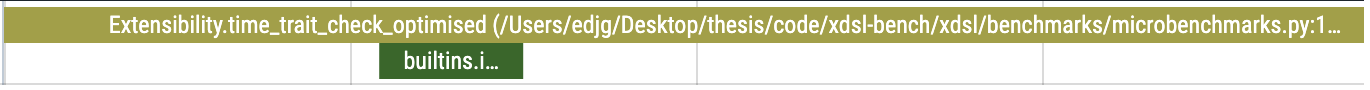
\includegraphics[width=\textwidth]{images/14_understanding_compiler_performance/trait_checks/hastrait_xdsl_viztracer_optimised.png}
        \caption{\texttt{viztracer} trace of xDSL's optimised \mintinline{python}{has_trait} implementation.}
        \label{fig:ubenchmark-hastrait-xdsl-viztracer-optimised}
    \end{subfigure}
    \begin{subfigure}[b]{\textwidth}
        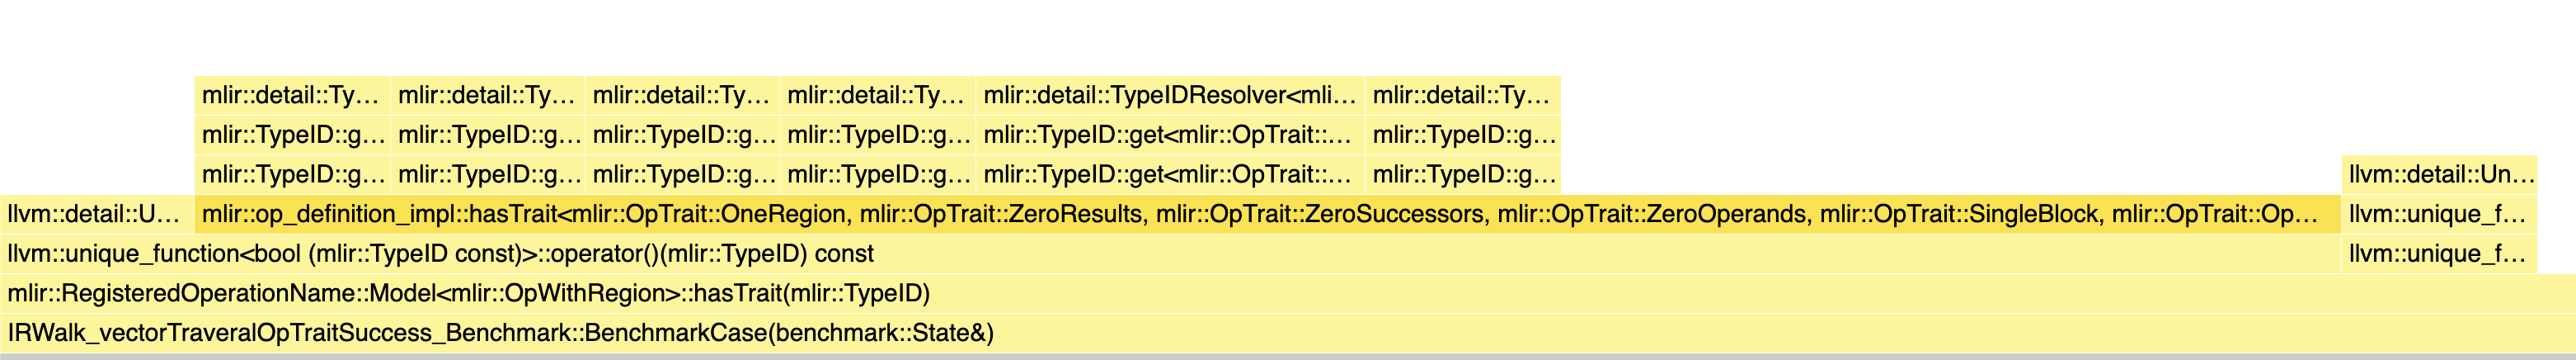
\includegraphics[width=\textwidth]{images/14_understanding_compiler_performance/trait_checks/hastrait_mlir_samply.png}
        \caption{\texttt{samply} trace of MLIR's \mintinline{c++}{has_trait} method.}
        \label{fig:ubenchmark-hastrait-mlir-samply}
    \end{subfigure}
    \caption{MLIR's dynamic trait checking using C++ RTTI is more complex than xDSL's Python implementation using \mintinline{python}{isinstance}.}
    \label{fig:ubenchmark-hastrait-dynamism}
\end{figure}
